\documentclass[convert]{standalone}
\usepackage{tikz}
\usetikzlibrary{arrows, backgrounds, calc, fit, positioning, shapes.geometric}
\pagecolor[RGB]{255,255,254}
\begin{document}
 \ifstandalone
  \def\imgpath{./}
 \else
  \def\imgpath{research/apets/}
 \fi
 \begin{tikzpicture}[>=stealth', relative=false]
  \def\r{2}
  \node at (180:\r) (E) {Evolution};

  \path (90:\r) ++(-.75, -.75)
    node (e) [font=\tiny] {Evaluation}
    -- ++(1.5, 0)
    node (et) [shape=diamond, draw, inner sep=1pt, font=\tiny] {A}
    -- ++(-.75, 1)
    node (t) [font=\tiny] {Learning};
  \draw [->] (e) to (et);
  \draw [->] (et) to (t);
  \draw [->] (t) to (e);
  \node (Einner) [fit=(e)(et)(t)] {};

  \draw [->] (E) to [out=90, in=180] (Einner);

  \node (S) at (0:\r) [shape=diamond, draw, inner sep=2pt] {B};
  \draw [->] (Einner) to [out=0, in=90] (S);

  \node (F) at (270:\r) [draw, font=\small] {Feedback};
  \draw [->] (S) to [out=-90, in=0] (F);
  \draw [->] (F) to [out=180, in=-90] (E);

%   \draw [red] (0,0) circle (\r);

  \node [right=.5 of S] (ps) {Pre-selection};
  \draw [->] (S) -- (ps);

  \node [right=1.5 of ps] (es_center) {};

  \foreach \a/\img in {south west/boxer_inv_simu, north west/boxer_simu,
                       south east/handball_player, north east/hammer_man} {
   \node at (es_center) (ind \a) [anchor=\a, inner sep=.1pt] {\includegraphics[width=1cm]{\imgpath/\img}};
   \draw [->] (ps) |- (ind \a);
  }

  \draw [red] (ind north west.north west) rectangle (ind north west.south east);

  \node (f) at (ps|-F) [shape=diamond, draw, inner sep=2pt] {C};
  \draw [->] (ind north west) to [out=270, in=0] (f);
  \draw [->] (f) to (F);

  \node (A) [below=.5 of f] {Assembly};
  \path (A-|es_center) ++ (0, -1) node (I) {Interaction};

  \draw [->] (I) to [out=315, in=225, loop below] node [pos=.25, font=\tiny] (a) {Learning} (I);

  \draw [->] (f) to (A);
  \draw [->] (A) to [out=0, in=90] node [pos=.5] {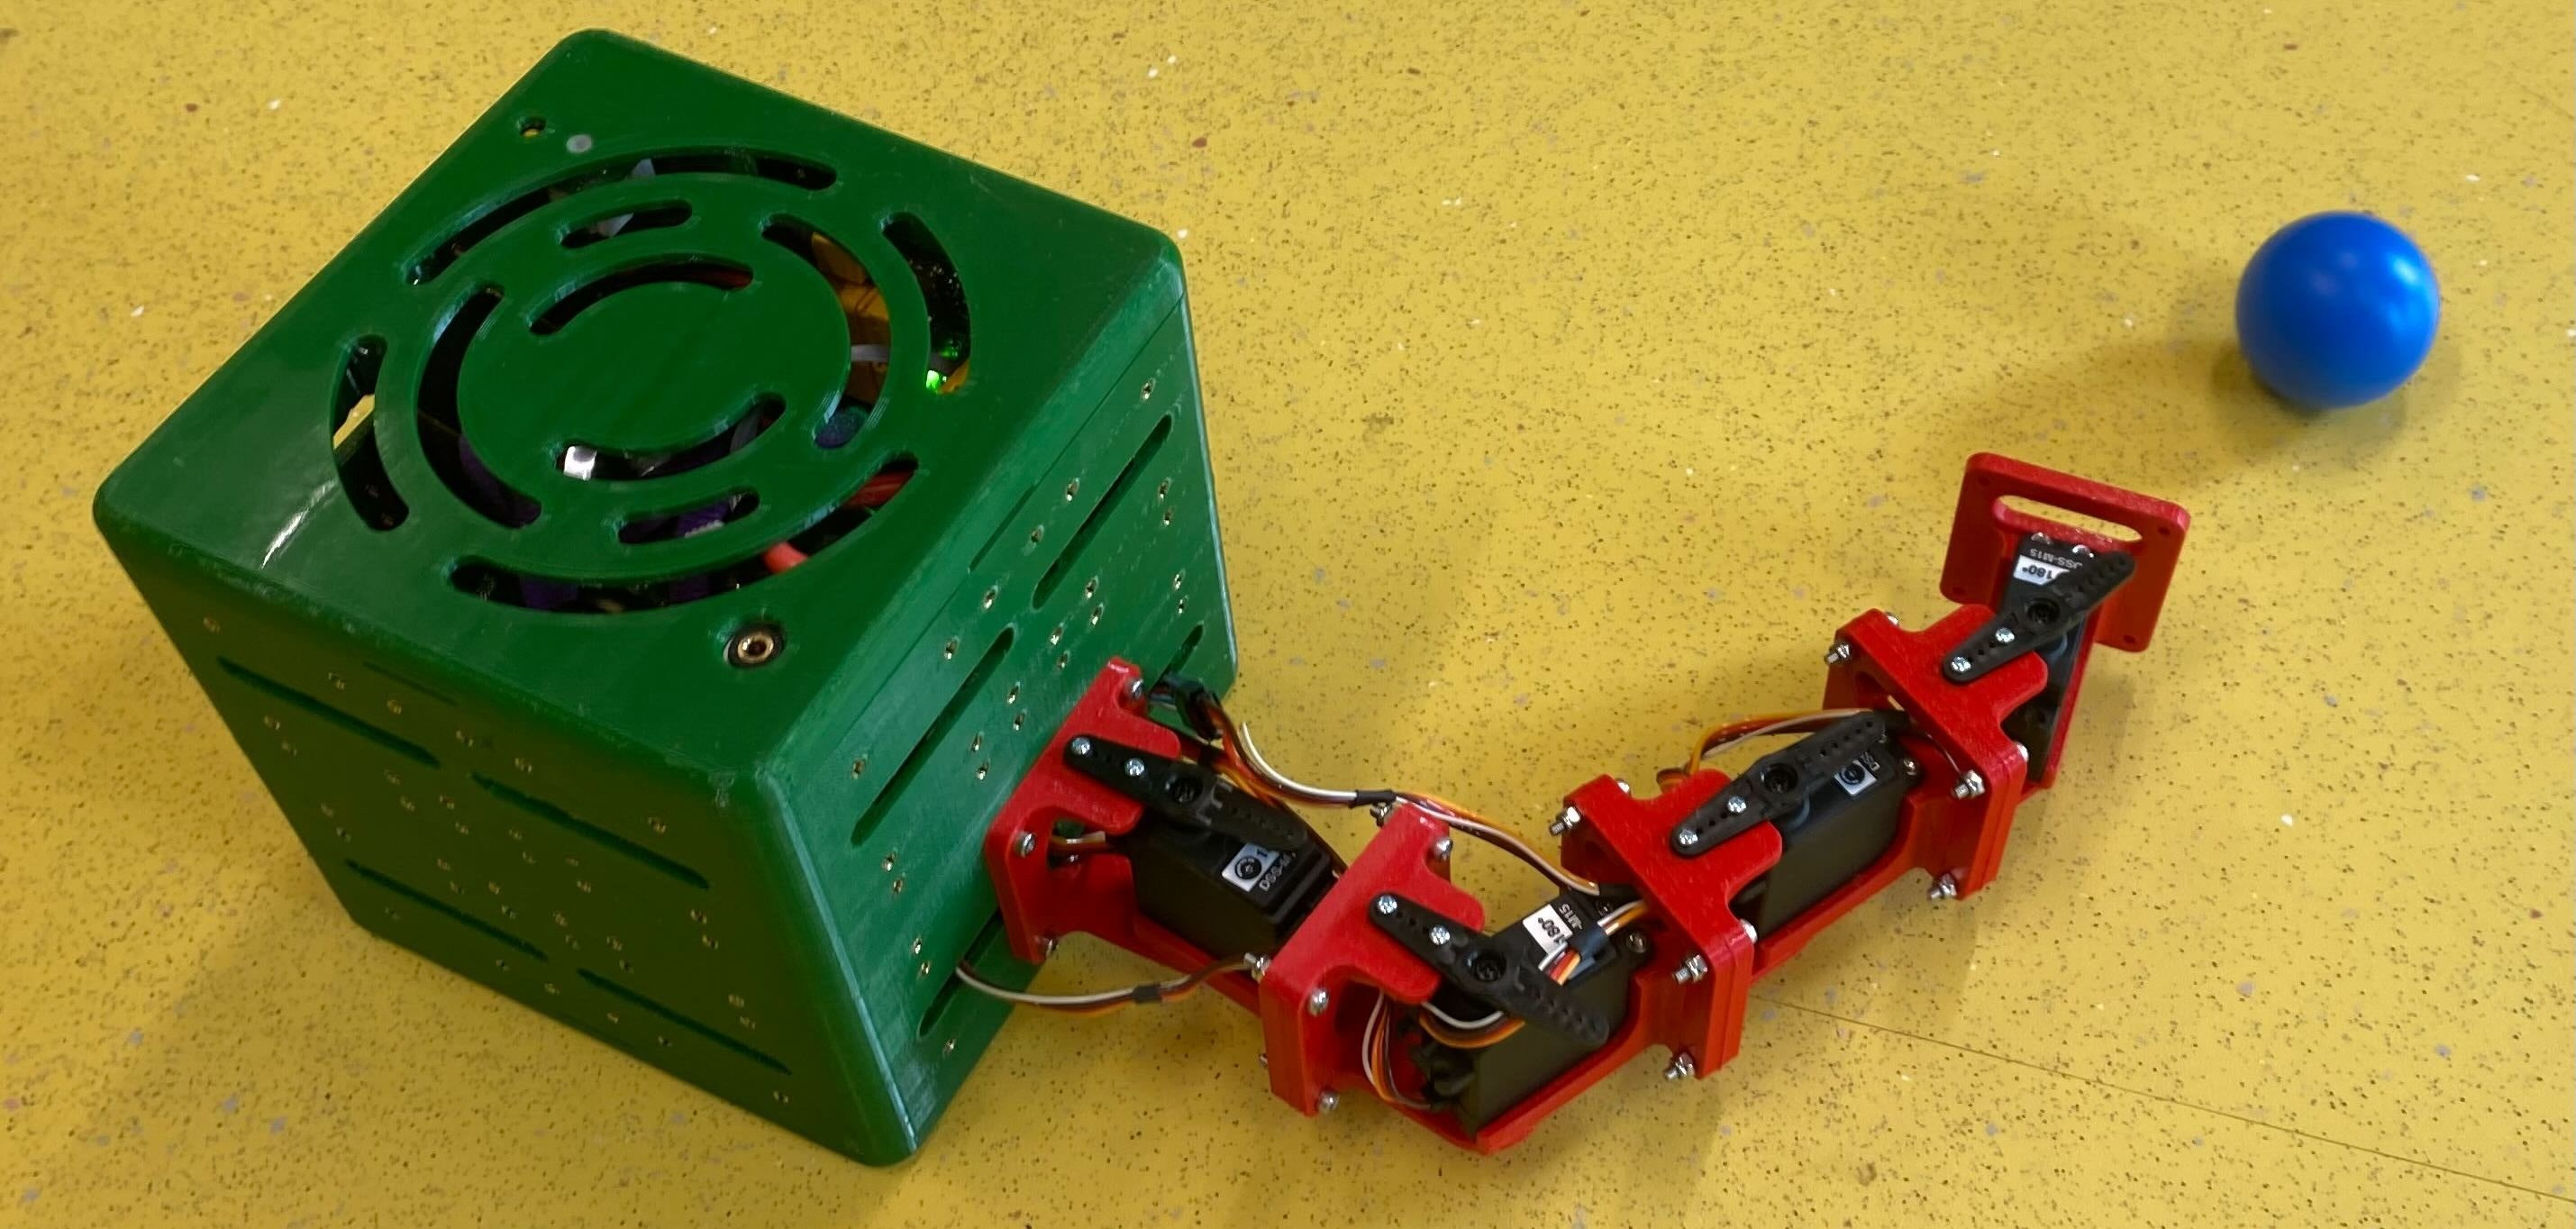
\includegraphics[width=1cm]{\imgpath/boxer_phys}}
                    (I);

  \node (D) at (F|-I) [shape=diamond, draw, inner sep=2pt] {D};
  \draw [->] (I) to (D);
  \draw [->] (D) to (F);
  \draw [->] (D) -| ++(-1.5, .5) node [anchor=south] {Deployment};

  \coordinate (middle) at ($(ps)!.5!(es_center)$);
  \coordinate (top) at (middle|-current bounding box.north);
  \coordinate (bottom) at (middle|-current bounding box.south);

  \node [below left=0 of top, draw, inner sep=5pt] {\textbf{Simulation}};
  \node [below right=0 of top, draw, inner sep=5pt] {\textbf{Human}};

  \node (W) [dashed, draw, fit=(A)(I)(a), inner sep=5pt] {};
  \node (Wlabel) at (W.south-|bottom.south) [anchor=south, draw, inner sep=5pt] {\textbf{World}};

  \draw [dashed] (top) to (Wlabel);

  \begin{scope}[on background layer]
   \fill [green, fill opacity=.1] (top) rectangle (current bounding box.south west);
   \fill [blue, fill opacity=.1] (top) rectangle (current bounding box.south east);
   \fill [red, fill opacity=.1] (W.north east) rectangle (W.south west);

  \end{scope}
 \end{tikzpicture}
\end{document}
